\chapter{Chapter Name} 

Chapter introduction

\section{Section 1}
\label{sec:sec-1}

Citation ~\cite{s:source1}.

Reference to section 1: \ref{sec:sec-1}

\begin{table}[h]
\centering
\caption{Energy use in the US food system as a percentage of total domestic energy}
\label{tab_agric_energy}
\vspace{6pt}
\begin{tabular}{lcccc}
\toprule
Process & \multicolumn{3}{c}{Study} & Average \\
\cmidrule(r){2-4}
 & Fluck & Singh & Poincelot & \\
\midrule
Production & 55.36  & 62.86 & 62.86 & 60.36 \\
Wholesale/Retail & 28.93    & 28.21 & 9.29  & 22.14 \\
Transport & 46.43   & 8.57  & 28.21 & 27.74 \\
\midrule
\midrule
Total domestic energy (\%) & 4.51   & 4.62  & 4.76  & 4.63 \\
\bottomrule
\end{tabular}
\end{table}

Table \ref{tab_agric_energy} reference.

\section{Section 2}
\label{sec:sec-2}

Descriptions:

\begin{description}

\item[Item 1]
Descript

\item[Item]
asdf. Cite 2 ~\cite{s:source2}

\end{description}

\section{Section 3}

asdf

\subsection{Sub section}

Some more stuff

\subsubsection{Sub section}

Even more, with a figure:

\begin{figure}[h]
    \centering
    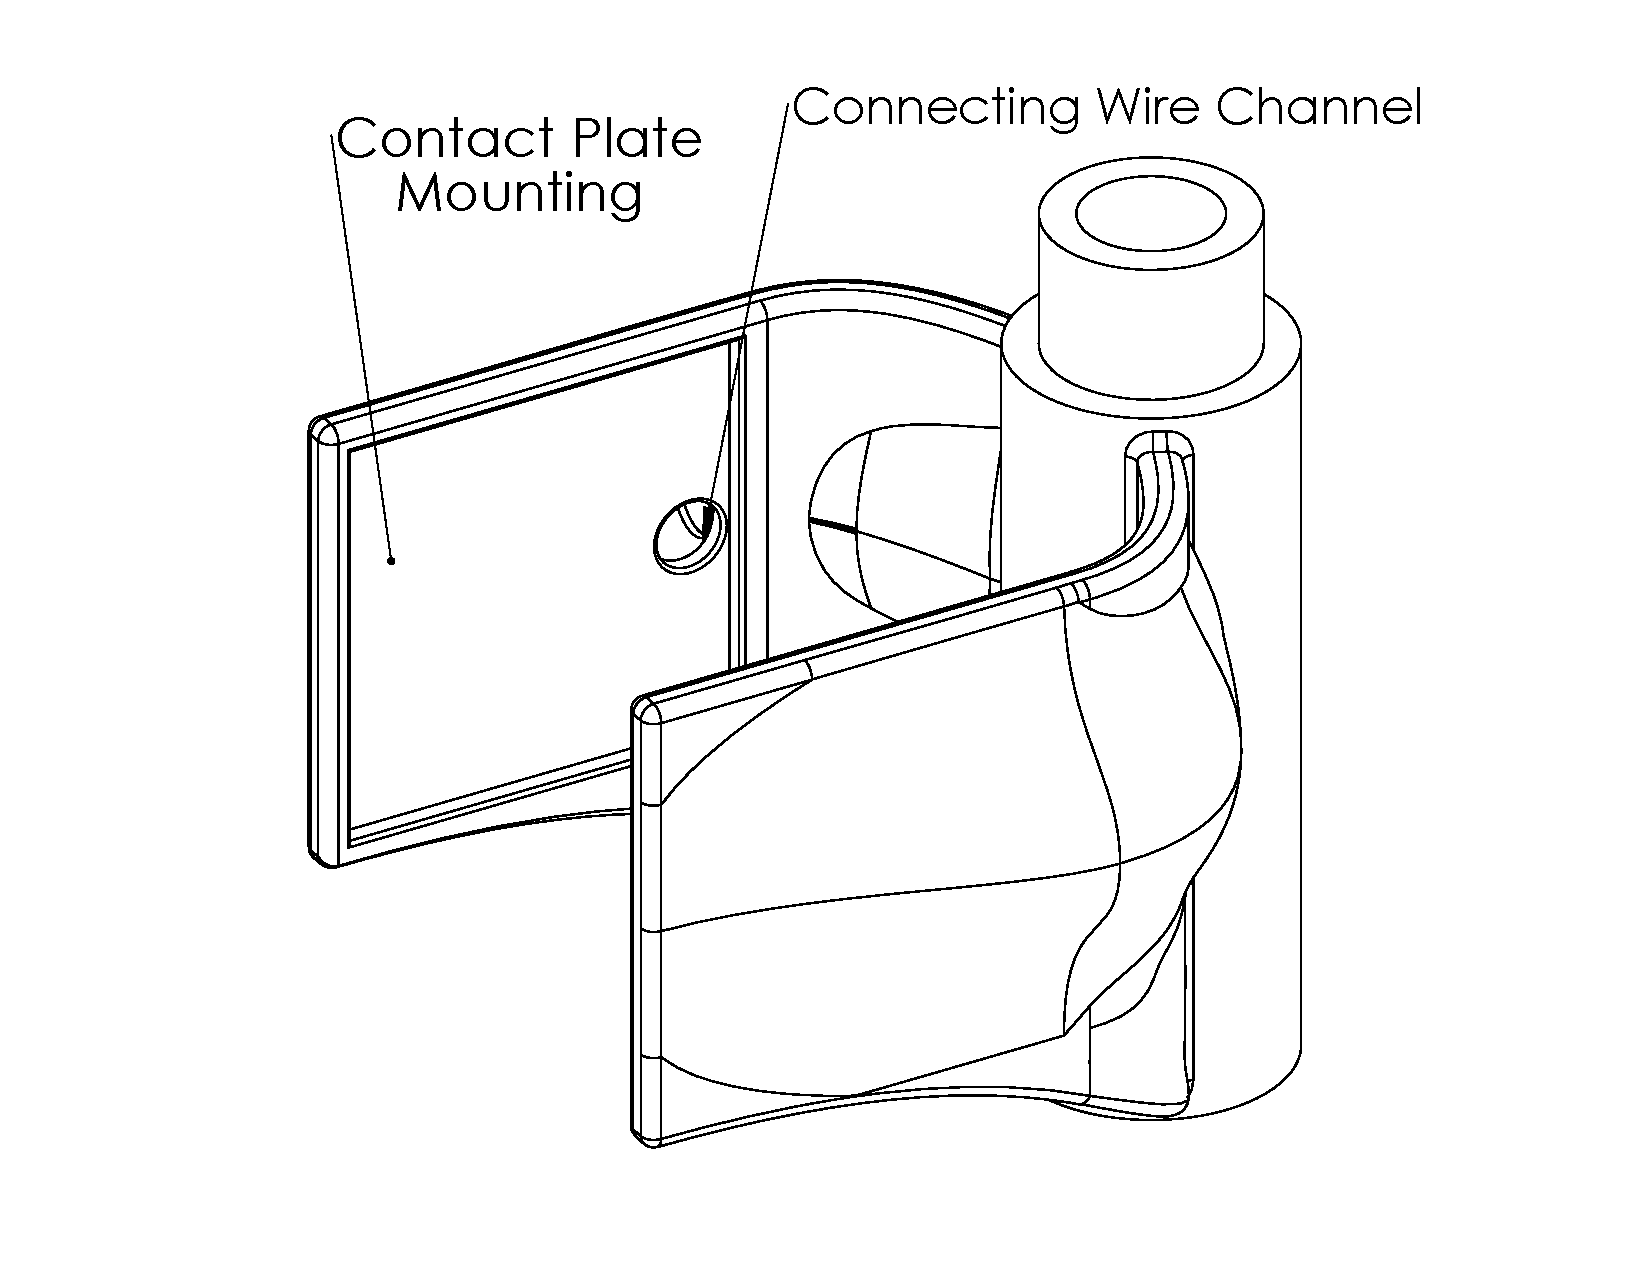
\includegraphics[width=.5\textwidth]{images/MoistureSensor}
    \caption{Custom Moisture Sensor}
    \label{fig:moistureSensor}
\end{figure}

And to reference figure \ref{fig:moistureSensor}